% !TEX TS-program = xelatex
% !TEX encoding = UTF-8 Unicode
\input{../structure.tex}

\title{Problems in higher dimensions}
\subtitle{Some examples on how things generalize beyond 1d}
\date{16/2/2021}
\date{}
%\author{18.303 Linear Partial Differential Equations: Analysis and Numerics}
\institute{18.303 Linear Partial Differential Equations: Analysis and Numerics}
\titlegraphic{\hfill\includegraphics[height=2em]{../MIT-logo.pdf}}

\begin{document}
	
	\maketitle
	
%	\begin{frame}{Table of contents}
%		\setbeamertemplate{section in toc}[sections numbered]
%		\tableofcontents%[hideallsubsections]
%	\end{frame}

\begin{frame}{Poisson equation in 2d}
	Consider a box of size $(L_x,L_y)$ with periodic boundaries.
	\metroset{block=fill}
	\begin{block}{\centering Poisson's equation with periodic boundaries}
		\begin{align*}
			\Delta u(x,y) &= \pfrac[2]{u(x,y)}{x} + \pfrac[2]{u(x,y)}{y} = f(x,y); \\
			u(0,y) &= u(L_x,y), \; u(x,0)=u(x,L_y) 
		\end{align*}
	\end{block}
	We require that $(x,y) \in \Omega = [0,L_x]\times [0,L_y]. $
\end{frame}


\begin{frame}
	\begin{figure}
		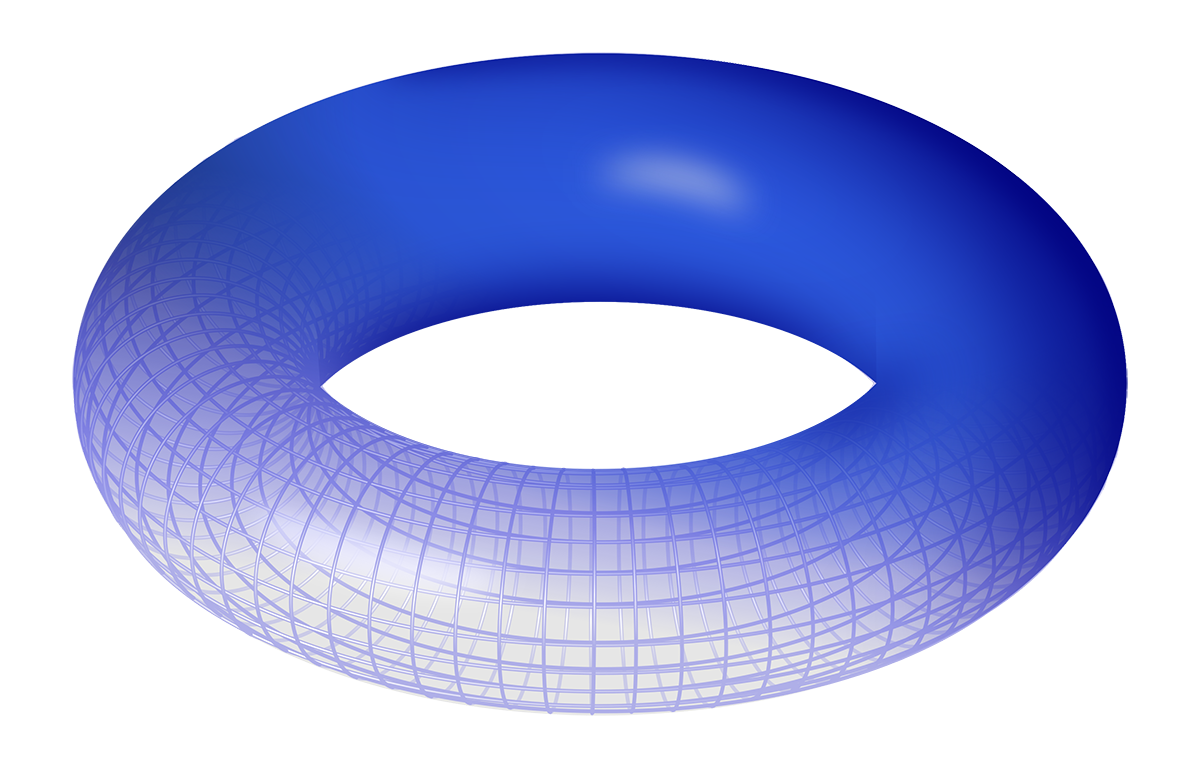
\includegraphics[width=0.9\linewidth]{torus.png}
		\caption{How $ \Omega $ looks like (topologically).}
	\end{figure}
\end{frame}

\begin{frame}
	\metroset{block=fill}
	\begin{block}{\centering Poisson's equation with periodic boundaries}
		\begin{align*}
			\Delta u(x,y) &= \pfrac[2]{u(x,y)}{x} + \pfrac[2]{u(x,y)}{y} = f(x,y); \\
			u(0,y) &= u(L_x,y), \; u(x,0)=u(x,L_y); \\
			u_x(0,y) &= u_x(L_x,y), \; u_y(x,0)=u_y(x,L_y). 
		\end{align*}
	\end{block}
(Here $ u_x = \partial_x u$ and $ u_y = \partial_y u$).

\pause
How do we solve this?
\end{frame}

\begin{frame}
	As we did before, let's try finding the eigenfunctions in order to invert the Laplacian. This gives
	the eigenvalue problem
	
	\pause
	\metroset{block=fill}
	\begin{block}{\centering Eigenproblem for the Laplacian with periodic boundaries}
		\begin{align*}
			 \pfrac[2]{\eigone\argtwo}{x} &+ \pfrac[2]{\eigone\argtwo}{y} = -\lambda_\vn^2 \eigone\argtwo; \\
			\eigone(0,y) &= \eigone(L_x,y), \; \eigone(x,0)=\eigone(x,L_y); \\
			\eigone_x(0,y) &= \eigone_x(L_x,y), \; \eigone_y(x,0)=\eigone_y(x,L_y). 
		\end{align*}
	\end{block}
	
	\pause
	We can again try out a solution that is separable. Let $ \eigone\argtwo = X_n(x)Y_m(y) $. This gives
	\[  
	Y_m(y) X_n''(x) + X_n(x) Y_m''(y) = -\lambda_{n,m}^2 X_n(x) Y_m(y).
	\]
	
	\pause
	Dividing by $XY$ gives
	\[  
	\frac{X_n''(x)}{X_n(x)} + \frac{Y_m''(y)}{Y_m(y)} = -\lambda_{n,m}^2.
	\]
\end{frame}

\begin{frame}
	This is again possible only if 
	\[  
	\begin{split}
		X_n''(x) &= -\mu_n^2 X_n(x), \\
		Y_m''(y) &= -\nu_m^2 Y_m(y).
	\end{split}
	\]
	
	\pause
	Before proceeding with the calculation, let's talk about the boundary conditions. We have 
	\[  
	\begin{split}
		\eigone(0,y) &= \eigone(L_x,y), \; \eigone(x,0)=\eigone(x,L_y); \\
		\eigone_x(0,y) &= \eigone_x(L_x,y), \; \eigone_y(x,0)=\eigone_y(x,L_y). 
	\end{split}
	\]
	
	\pause
	Substituting $\eigone = X_n Y_m$ gives
	\[  
	\begin{split}
		X_n(0) &= X_n(L_x), \; Y_m(0)=Y_m(L_y); \\
		X_n'(0) &= X_n'(L_x), \; Y_m'(0)=Y_m'(L_y)
	\end{split}
	\]
	i.e. we have periodic boundary conditions for both $X_n$ and $Y_m$. 
\end{frame}

\begin{frame}
	We see that the problem separates nicely. We have two unrelated eigenvalue problems for $X_n$ and $Y_m$. Let's solve one of these explicitly since we haven't done that in class.
	
	\pause
	We know that $X_n(x) = \exp(i\mu_n x)$ and we require 
	\[  
	X_n(0) = X_n(L_x) \Leftrightarrow 1 = \exp(i\mu_n L_x).
	\]
	This gives 
	\[  
	\mu_n = \frac{2\pi n}{L_x},
	\]
	where $ n\in \Z $. 
	
	\pause
	Similarly, we get 
	\[  
	Y_m(y) = \exp(i \nu_m x),
	\]
	where $ \nu_m = 2\pi m/L_y $. One should mention that we have $ \lambda_{n,m}^2 = \mu_n^2 + \nu_m^2 $.
	
	\pause
	Now, the solution can be expressed as 
	\[  
	u(x,y) = \sum_{n=-\infty}^{\infty} \hat{X}_n e^{2\pi i n x/L_x} \sum_{m=-\infty}^{\infty} \hat{Y}_m e^{2\pi i m x/L_x} = \sum_{n,m=-\infty}^{\infty} \hat{X}_n \hat{Y}_m e^{2\pi i (nx/L_x+my/L_y) }.
	\]
\end{frame}

\begin{frame}
	We get new Fourier coefficients that depend on two indices. We can write $ u $ now as 
	\begin{equation}\label{eq:fourier_expansion}
		u(x,y) = \sum_{n,m=-\infty}^{\infty} \hat{u}_{n,m} e^{2\pi i (nx/L_x+my/L_y) }.
	\end{equation}
	
	\pause
	Taking the differential operator of $ u $ gives
	\[  
	\begin{split}
	\sum_{n,m=-\infty}^{\infty} \hat{u}_{n,m} &\left(\pfrac[2]{}{x} + \pfrac[2]{}{y} \right)e^{2\pi i (nx/L_x+my/L_y) } =  \\
	&-\sum_{n,m=-\infty}^{\infty} \hat{u}_{n,m} \left[
	\left(\frac{2\pi n}{L_x} \right)^2 + \left(\frac{2\pi m}{L_y}\right)^2 
	\right]
	e^{2\pi i (nx/L_x+my/L_y) }.
	\end{split}
	\]
\end{frame}

\begin{frame}
	This gives us 
	\begin{equation}\label{eq:Poisson_solution}
		-\sum_{n,m=-\infty}^{\infty} \hat{u}_{n,m} \left[
		\left(\frac{2\pi n}{L_x} \right)^2 + \left(\frac{2\pi m}{L_y}\right)^2 
		\right]
		e^{2\pi i (nx/L_x+my/L_y) } = f\argtwo . 	
	\end{equation}
	
	\pause
	We continue as before. We can show that the eigenfunctions $ \{ \eigone \}_\vn $, where $ \vn = (n,m) $ are orthogonal. 
	
	\pause
	This can be expressed as 
	\[  
	\iprod{\phi^{(n,m)}}{\phi^{(j,k)}} = \int_0^{L_x} \int_{0}^{L_y} e^{2\pi i ((j-n)x/L_x + (k-m)y/L_y)} \diff x \diff y = \delta_{j,n} \delta_{k,m} L_x L_y
	\] 
	i.e. it gives $ L_x L_y $ if $ j=n $ and $ k=m $ and zero otherwise. 
	
	\pause 
	\textbf{Exercise}: Show this.
\end{frame}

\begin{frame}
	Now we get the coefficients 
	\[  
	\hat{u}_{n,m} = -\frac{\iprod{\phi^{(n,m)}}{f}}{ L_x L_y \lambda_{n,m}^2} 
	= -\frac{\hat{f}_{n,m}}{  \lambda_{n,m}^2},
	\]
	where 
	$$ 
	\lambda_{n,m}^2 = \left(\frac{2\pi n}{L_x} \right)^2 + \left(\frac{2\pi m}{L_y} \right)^2. 
	$$
	
	\pause
	What if $ \lambda_{n,m} = 0 $? This actually happens for $ n,m=0 $. This corresponds to the eigenfunction $ \exp(0) = 1 $ i.e. the constant part of the function. For periodic domains constant solutions are always in the null space of the Laplacian operator. Some extra information is needed to get this. 
	
	\pause
	What we often know is the value of 
	\[ \int_{\Omega} u (\varone) \diff \varone = \hat{u}_{0,0}L_x L_y. \]
	Here $ \varone = (x,y) $ and $ \Omega $ is given by the box.
	
	\pause
	\textbf{Question:} Why do we have the latter equality?
	
\end{frame}

\begin{frame}{Fourier coefficients}
	We get the coefficients as
	\begin{equation}\label{eq:fourier_transform}
		\hat{f}_\vn = \frac{1}{\mu(\Omega)}\int_{\Omega}  \exp \left( - i \vk_\vn \cdot \vec{x} \right) f(\varone) \diff \varone,
	\end{equation}
	where $ \vn = (n_x,n_y) $ and $ \vk_{\vn} = 2\pi (n_x/L_x,n_y/L_y) $. The function $ \mu(\Omega) = L_x L_y $
	gives the "volume" of the space. 
	
	\pause
	As we briefly discussed earlier, this defines a formal linear transformation $ \fouriert $ that takes functions from one vector space to another. We can write $ \hat{f}_\vn = \fouriert(f)_\vn $.
	
	\pause
	The inverse transform gives back $ f $ i.e. $ \fouriert^{-1} (\hat{f}) (x) = f(x) $. This is also given by 
	\[  
	f(x) = \sum_{\vn\in \Z^2} \hat{f}_\vn \exp(i \vk_{\vn} \cdot \varone).
	\]
	
	In literature $ \fouriert $ is sometimes called the \alert{finite Fourier transform}. We will talk about the actual Fourier transform later on.
\end{frame}

\begin{frame}
	What if $ f $ is real?
	
	\pause
	For the (finite) Fourier transform it doesn't really matter but we get a nice relation. Because for real functions we have $ f(x)^* = f(x) $, the Fourier expansion gives 
	\[  f(x)^* = f(x) \Leftrightarrow
	\sum_{\vn\in \Z^2} \hat{f}_\vn^* \exp(-i \vk_{\vn} \cdot \varone)
	= \sum_{\vn\in \Z^2} \hat{f}_\vn \exp(i \vk_{\vn} \cdot \varone)
	= \sum_{\vn\in \Z^2} \hat{f}_{-\vn} \exp(-i \vk_{\vn} \cdot \varone).
	\]
	
	\pause
	Because the basis is orthogonal, the coefficients have to be the same. This gives
	\[  
	\hat{f}_{-\vn} = \hat{f}^*_{\vn}
	\]
	i.e. we only need to calculate, say, the coefficients with $ n_x \geq 0 $ and the ones corresponding to the negative indices are given by taking the complex conjugate of the coefficients corresponding to positive indices. The numerical algorithms using this fact are called \emph{real Fourier transforms} (\texttt{rfft}).  
	
\end{frame}

\begin{frame}{Exercise \exercisen}
	Assume that we have 1d Fourier expansion of a real function  
	\[  
	f(x) = \sum_{n=0}^{\infty} \alpha_{n} \sin(k_n x) + \beta_n \cos(k_n x) 
	=  \sum_{n=-\infty}^{\infty} \hat{f}_n \exp(i k_n x).
	\] 
	Whats the relation between $ \hat{f}_n $ and $\alpha_n$ and $\beta_n$?
\end{frame}

\begin{frame}{Heat equation}
	What about the heat equation with periodic boundaries?
	
	\pause
	We have 
	\[  
	\pfrac{}{t} u\argone = \Delta u\argone
	\]
	and the same spatial boundary conditions for all $ t $ and in addition we are given
	\[  
	u(0,\varone) = u^{(0)}(\varone).
	\]
	
	\pause
	We can actually solve this the same way we did before using the separation $ u\argone = T_\vn(t) X_\vn (\varone)$ but now the spatial part depends on two coordinates. 
	
\end{frame}

\begin{frame}
	As before we get 
	\[  
	\begin{split}
	T_{\vn}'(t) &= -\lambda_{\vn}^2 T_{\vn}(t), \\
	\Delta X_{\vn}(\varone) &= -\lambda_{\vn}^2 X_{\vn}(\varone).
	\end{split}
	\]
	
	\pause
	We know that 
	\[  
	T_{\vn}(t) = T_{\vn}^{(0)} \exp(-\lambda_{\vn}^2 t)
	\]
	\pause
	and that 
	\[  
	X_\vn = \exp(i \vk_{\vn}\cdot \varone ).
	\]
	(Also, in this notation $ \lambda_{\vn}^2 = |\vk_{\vn}|^2$.)
	
\end{frame}

\begin{frame}
	The solution is given by 
	\[  
	u\argone = \sum_{\vn\in \Z^2} T_{\vn}^{(0)} X_\vn \exp(-k_{\vn}^2 t),
	\]
	where the coefficients $ T_{\vn}^{(0)} $ are the same as the Fourier coefficients of the initial condition 
	\[  
	u^{(0)}(x) = \sum_{\vn\in \Z^2} \hat{u}^{(0)}_{\vn} X_{\vn}.
	\]
	
	\textbf{Remark:} remember that $ T_{0}^{(0)} $ is related to the average value of $ u $. This doesn't evolve in time, which tells us that the heat equation preserves the average value of $ u $. 
\end{frame}

\begin{frame}{Conclusion}
	\begin{itemize}[<+->]
		\item We saw how we can use separation of variables to solve problems in many dimensions
		\item \textbf{Warning:} this only works for highly symmetric cases as the box we considered today
		\item The heat equation example showed what I pointed out previously, namely that if you can solve the eigenproblem for the spatial part, solving for the time evolution is easy
		\item We briefly talked about finite Fourier transforms and how they can be used both for real and imaginary functions
	\end{itemize}
\end{frame}

\end{document}
